\documentclass[tikz,border=10pt]{standalone}
\usepackage{tikz}
\usetikzlibrary{positioning}

\begin{document}
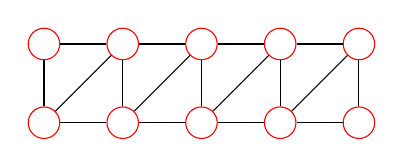
\begin{tikzpicture}[every node/.style={circle, draw, minimum size=4mm, color=red}]

% A replicated graph of Q5b.

\node (a) at (0,1) {};
\node (b) at (0,0) {};
\node (c) at (1,0) {};
\node (d) at (1,1) {};
\node (e) at (2,1) {};
\node (f) at (2,0) {};
\node (g) at (3,0) {};
\node (h) at (3,1) {};
\node (i) at (4,1) {};
\node (j) at (4,0) {};

\draw (a) -- (b) -- (c) -- (f) -- (g) -- (j) -- (i) -- (h) -- (e) -- (d) -- (a);
\draw (c) -- (d);
\draw (f) -- (e);
\draw (g) -- (h);

\draw (b) -- (d);
\draw (c) -- (e);
\draw (f) -- (h);
\draw (g) -- (i);

\end{tikzpicture}
\end{document}